% Emacs, this is -*-latex-*-
\documentclass[12pt]{ugentreport}
\usepackage[a4paper]{geometry}
\geometry{a4paper,margin=3cm,marginparwidth=20mm}
\usepackage[dutch]{babel}
\usepackage{parskip}
\usepackage{amsfonts}
\usepackage{amsmath}
\usepackage{cancel}
\usepackage{commath}
\usepackage{amssymb}
\usepackage{parskip}
\usepackage{rotating}
\usepackage{listings}
\usepackage{siunitx}
\usepackage{graphicx}
\usepackage{geometry}
\usepackage{underscore}
\usepackage{tikz}
\usepackage[dutch]{todonotes}
% Gives me \intertext and \shortintertext
\usepackage{mathtools}
\usepackage[european, siunitx]{circuitikz}
\usetikzlibrary{calc}
% Nicer unit fractions
\sisetup{per-mode=fraction}
% Smaller margins
% \usepackage{fullpage}
% Clickable links
\usepackage{hyperref}

\lstMakeShortInline[basicstyle=\ttfamily,language=C]{§}

\title{Verslag Project Microcontrollers}
\author{Marieke Louage\and Stef Pletinck}

\begin{document}

\maketitle

\tableofcontents
\listoffigures
\listoftodos
\newpage

\section{Doelstellingen}
Doel van deze opgave was het maken van een spel op een microcontroller,
specifiek een \emph{AT90USB646} op een \emph{Dwenguino} ontwikkelbord.
Verdere doelen van het vak zijn het leren lezen en interpreteren van datasheets
en werken met de taal \emph{C}.
Er werd besloten om een multiplayer spel te maken,
voor meer interactiviteit.

Voor de weergave van het spel werden verschillende mogelijkheden overlopen.
Een eerste mogelijkheid was het aansturen van een VGA-display,
maar door de hoge klokfrequentie van VGA en de daaraan gelinkte problemen
werd dit idee snel verworpen.
Een tweede idee was het gebruik van een LED-matrix.
De lage resolutie hiervan was echter een groot nadeel,
dus werd uiteindelijk gekozen voor een scherm dat gebruik maakt
van het principe van een hardeschijfklok. Een snel ronddraaiende ledstrip werd
ook overwogen, maar dit is praktisch niet haalbaar.

Het spel zelf vindt plaats in een baan rond de aarde, waar twee ruimteschepen
elkaar rond de aarde achtervolgen en proberen neer te schieten.

Als invoer van de spelers werd gekozen voor arcade-joysticks.
Deze bestaan uit vier microswitches per joystick.
Er waren verder nog vele ideeën om het spel verder uit te breiden.

\section{Praktische aanpak}
De nodige functionaliteit werd opgedeeld in logische blokken die met elkaar
communiceren en op elkaar vertrouwen voor informatie. De bekomen structuur is
zichtbaar in figuur~\ref{fig:structuur}.
Op deze figuur staat hardware in een ovaal en software in rechthoekjes.

Het motorsysteem staat los van alles, en genereert op basis van interrupts het
controlesignaal voor de hardwarematige motordriver, die de hardeschijfmotor
aanstuurt.

Een optische sensor genereert interrupts, die worden geïnterpreteerd tot
timinginformatie over de draaischijf. Deze worden gebruikt door het
\emph{graphics} systeem om de juiste LED's te laten oplichten. Dit systeem wordt
constant vanuit een lus in §main()§ opgeroepen, en geeft door welke LED's moeten
oplichten aan de \emph{leddriver}, die de feitelijke seriële data genereert en
blokkerend doorstuurt naar de LED's.

De gegevens voor het \emph{graphics} systeem worden gegenereerd door de
\emph{engine}, die via een interrupt 30 keer per seconde alle objecten in het
spel ververst en doorgeeft aan \emph{graphics}. Daarvoor worden gegevens over de
joysticks synchroon uitgelezen door het \emph{joysticks} systeem.

\begin{figure}
  \centering
  \includegraphics[width=0.8\textwidth]{img/structuur.jpg}
  \caption{Structuur van het microcontrollerprogramma}
  \label{fig:structuur}
\end{figure}


\subsection{Werking display}
Een schijf met gaten draait snel rond over LED's, verspreid in sectoren, zie figuur~\ref{fig:schijf}
Door de LED's op de gepaste momenten in en uit te schakelen
kan een zeer hoge resolutie bekomen worden rond het middelpunt.
In de radiale richting is de resolutie beperkt door het aantal LED's,
dit werd oorspronkelijk gekozen op 16 om de aansturing werkbaar te houden.
Er bleek dat er, door de dunne wanden tussen sectoren, soms twee ``pixels''
zich boven dezelfde sector bevonden en \emph{spookpixels} weergaven,
dus is het aantal sectoren behouden op 16,
maar werd besloten om in de radiale richting naar 13 pixels te gaan.

Met deze aanpak is het mogelijk om willekeurig de resolutie te kiezen
waarmee de hoek wordt beschreven. Hoe groter deze resolutie,
hoe meer pixels. Deze waarde werd gekozen op 1024, dit als een goede balans
tussen nauwkeurigheid van het display en haalbaarheid. Hoe hoger deze resolutie,
hoe sneller de LED's namelijk ververst moeten worden om te zorgen dat alle
objecten weergegeven worden.

\begin{figure}
  \centering
  \includegraphics[width=0.6\textwidth]{img/schijf.jpg}
  \caption{Schema van de draaischijf}
  \label{fig:schijf}
\end{figure}

\subsection{Aansturing LED's}
De gebruikte LED's zijn ledstrips van het type \texttt{APA102}.
Deze kunnen vrij eenvoudig via SPI data ontvangen.
Elke LED krijgt een pakket bestaande uit 32 bits, zie
figuur~\ref{fig:ledpakket}.
Deze data moet byte per byte en bit per bit verzonden worden over één datalijn,
met een kloksignaal.

De ledstrip luistert naar nieuwe commando's na een startpakket
bestaande uit 32 0-bits. Vervolgens moet,
zoals zichtbaar op figuur~\ref{fig:ledcontrol},
een pakket per LED verstuurd worden gevolgd door
nogmaals 32 bits om te zorgen dat alle data ver genoeg doorgeschoven is.
De waarde van deze bits is onbelangrijk,
maar 0 is handig om te voorkomen dat er een LED op volle helderheid wit licht
geeft wanneer er niet naar elke LED gegevens worden gestuurd.

\begin{figure}
  \centering
  \includegraphics[width=0.6\textwidth]{img/ledpakket.png}
  \caption{Schema van een led-pakket}
  \label{fig:ledpakket}
\end{figure}

\begin{figure}
  \centering
  \includegraphics[width=0.8\textwidth]{img/ledcontrol.png}
  \caption{Schema van het aansturen van een ledstrip}
  \label{fig:ledcontrol}
\end{figure}

Er zijn twee mogelijke manieren om meerdere bytes te versturen over SPI,
via een blokkerende §while§-lus en via een interrupt.
Het is echter ook mogelijk om een interrupt te ontvangen wanneer een byte is
verzonden,
om vervolgens een volgende byte te verzenden. Op die manier kan CPU-tijd
uitgespaard worden, maar dit blijkt zeer lastig foutloos te implementeren.
Het spel gebruikt bijgevolg voorlopig nog de \emph{blocking} aanpak.

Het is handig om te weten wat de maximale frequentie is waarmee alle LED's
kunnen aangestuurd worden.
Hiervoor is het belangrijk te weten dat de microcontroller
een werkfrequentie heeft van \SI{16}{\mega\hertz}
en er maximaal 1 bit per 2 klokcycli kan verstuurd worden over SPI.
Er zijn 16 LED's, dit geeft een maximale frequentie van \SI{15625}{\hertz}.
In de praktijk zal deze limiet dus waarschijnlijk nooit een probleem leveren.

\subsection{Timing LED's}
\label{sec:ledtiming}
\todo{Meer uitleg over leds}
De juiste LED's moeten op correcte momenten aan en uit geschakeld worden
om op de juiste plaats op de cirkel pixels op te laten lichten,
en niet te lang zodat de pixels geen lijnen worden en alle mogelijke hoeken
bereikt worden.

Het \emph{graphics} systeem wordt daartoe zo snel mogelijk na elkaar opgeroepen
in een lus in §main()§. In deze §render()§ functie, wordt voor elke
\emph{entity} (bv. spelers, kogels, \dots) gecontroleerd of deze zich momenteel
onder een gaatje in de schijf bevindt, en onder welk gat. Als dit zo is, wordt
dit object omgezet in LED-informatie en krijgt de juiste LED deze waarden
toegekend. De §Led§ struct die daarvoor wordt gebruikt bevat informatie over de
algemene helderheid en hoeveelheid blauw, groen en rood.

De controle of een object weergegeven kan worden is niet exact, er zit een
lichte marge op de hoek om te voorkomen dat een tijdelijke vertraging in de code
objecten laat verdwijnen. Op de straal is er geen zulke marge, aangezien deze
slechts een klein aantal vaste waarden kan aannemen. Het \emph{graphics}-systeem
heeft de hoek waaronder de schijf staat nodig om deze controle uit te kunnen
voeren. Het systeem rekent dit zelf uit, gebaseerd op de tijd die nodig is voor
één volledige rotatie van de schijf, en de tijd sinds de schijf laatst het
nulpunt is gepasseerd. Deze waarden krijgt het uit de code die informatie
verzamelt uit de optische sensor.

\subsection{Fysieke constructie}
\todo{Waarom vierkante pixels?}
De fysieke constructie is een rechtstaand licht hellend display met voldoende
ruimte voor de elektronica en bedrading. De gehele constructie werd ontworpen
in het CAD-pakket Siemens NX 11 en voornamelijk uitgesneden op een lasercutter,
op een paar uitzonderingen na.

De draaischijf is op de lasercutter gemaakt en bestaat uit \SI{2}{\milli\meter} dikke zwarte ABS.
De schijf bevat 13 gaatjes, goed voor een straalresolutie van 13 pixels. De pixels
zijn gerangschikt in twee spiralen opdat buren veraf van elkaar zouden liggen. Zo
wordt de lichtvervuiling in een aangrenzend segmenten minimaal benadrukt door
zover mogelijk verwijderd te zijn van een sprite.

De segmenten zijn met een breekmes op een snijplank gemaakt uit een wit PVC vel.
Er zijn 16 segmenten en elk segment heeft één led die gemonteerd is op een wand
van de behuizing grenzend aan de cirkel. Het wit plastic zorgt voor een goede
diffusie van het licht van de ledjes.

Dat het aantal segmenten en gaten niet gelijk is aan elkaar komt doordat geen
twee gaten zich tegelijkertijd in hetzelfde segment mogen bevinden. Waarom bij
16 segmenten voor 13 gaten gekozen is wordt duidelijk gemaakt in figuur~\ref{fig:duiding1316}. De
rood aangeduide stukjes staan ter hoogte van het binnenste gaatje en zijn even
lang, de oranje lijnen zijn tonen de segmenten.

\begin{figure}
  \centering
  \includegraphics[width=0.6\textwidth]{img/16vs13.jpg}
  \caption{Duiding 16 segmenten 13 gaten}
  \label{fig:duiding1316}
\end{figure}

De sensorhouder is een klein ge-3D-print stuk dat de sensor op zijn plaats
houdt. Dit is zichtbaar in figuur~\ref{fig:sensorhouder}.

De behuizing is gemaakt uit 3mm dik MDF plaatmateriaal en is volledig demonteerbaar.
Op de behuizing kan een scherm uit een 3mm dikke plexiplaat geplaats worden. De plaat is te zien in figuur~\ref{fig:plexiplaat}.

\begin{figure}
  \centering
  \includegraphics[width=0.6\textwidth]{img/SensorHouder.jpg}
  \caption{ge-3D-printe sensorhouder}
  \label{fig:sensorhouder}
\end{figure}

\begin{figure}
  \centering
  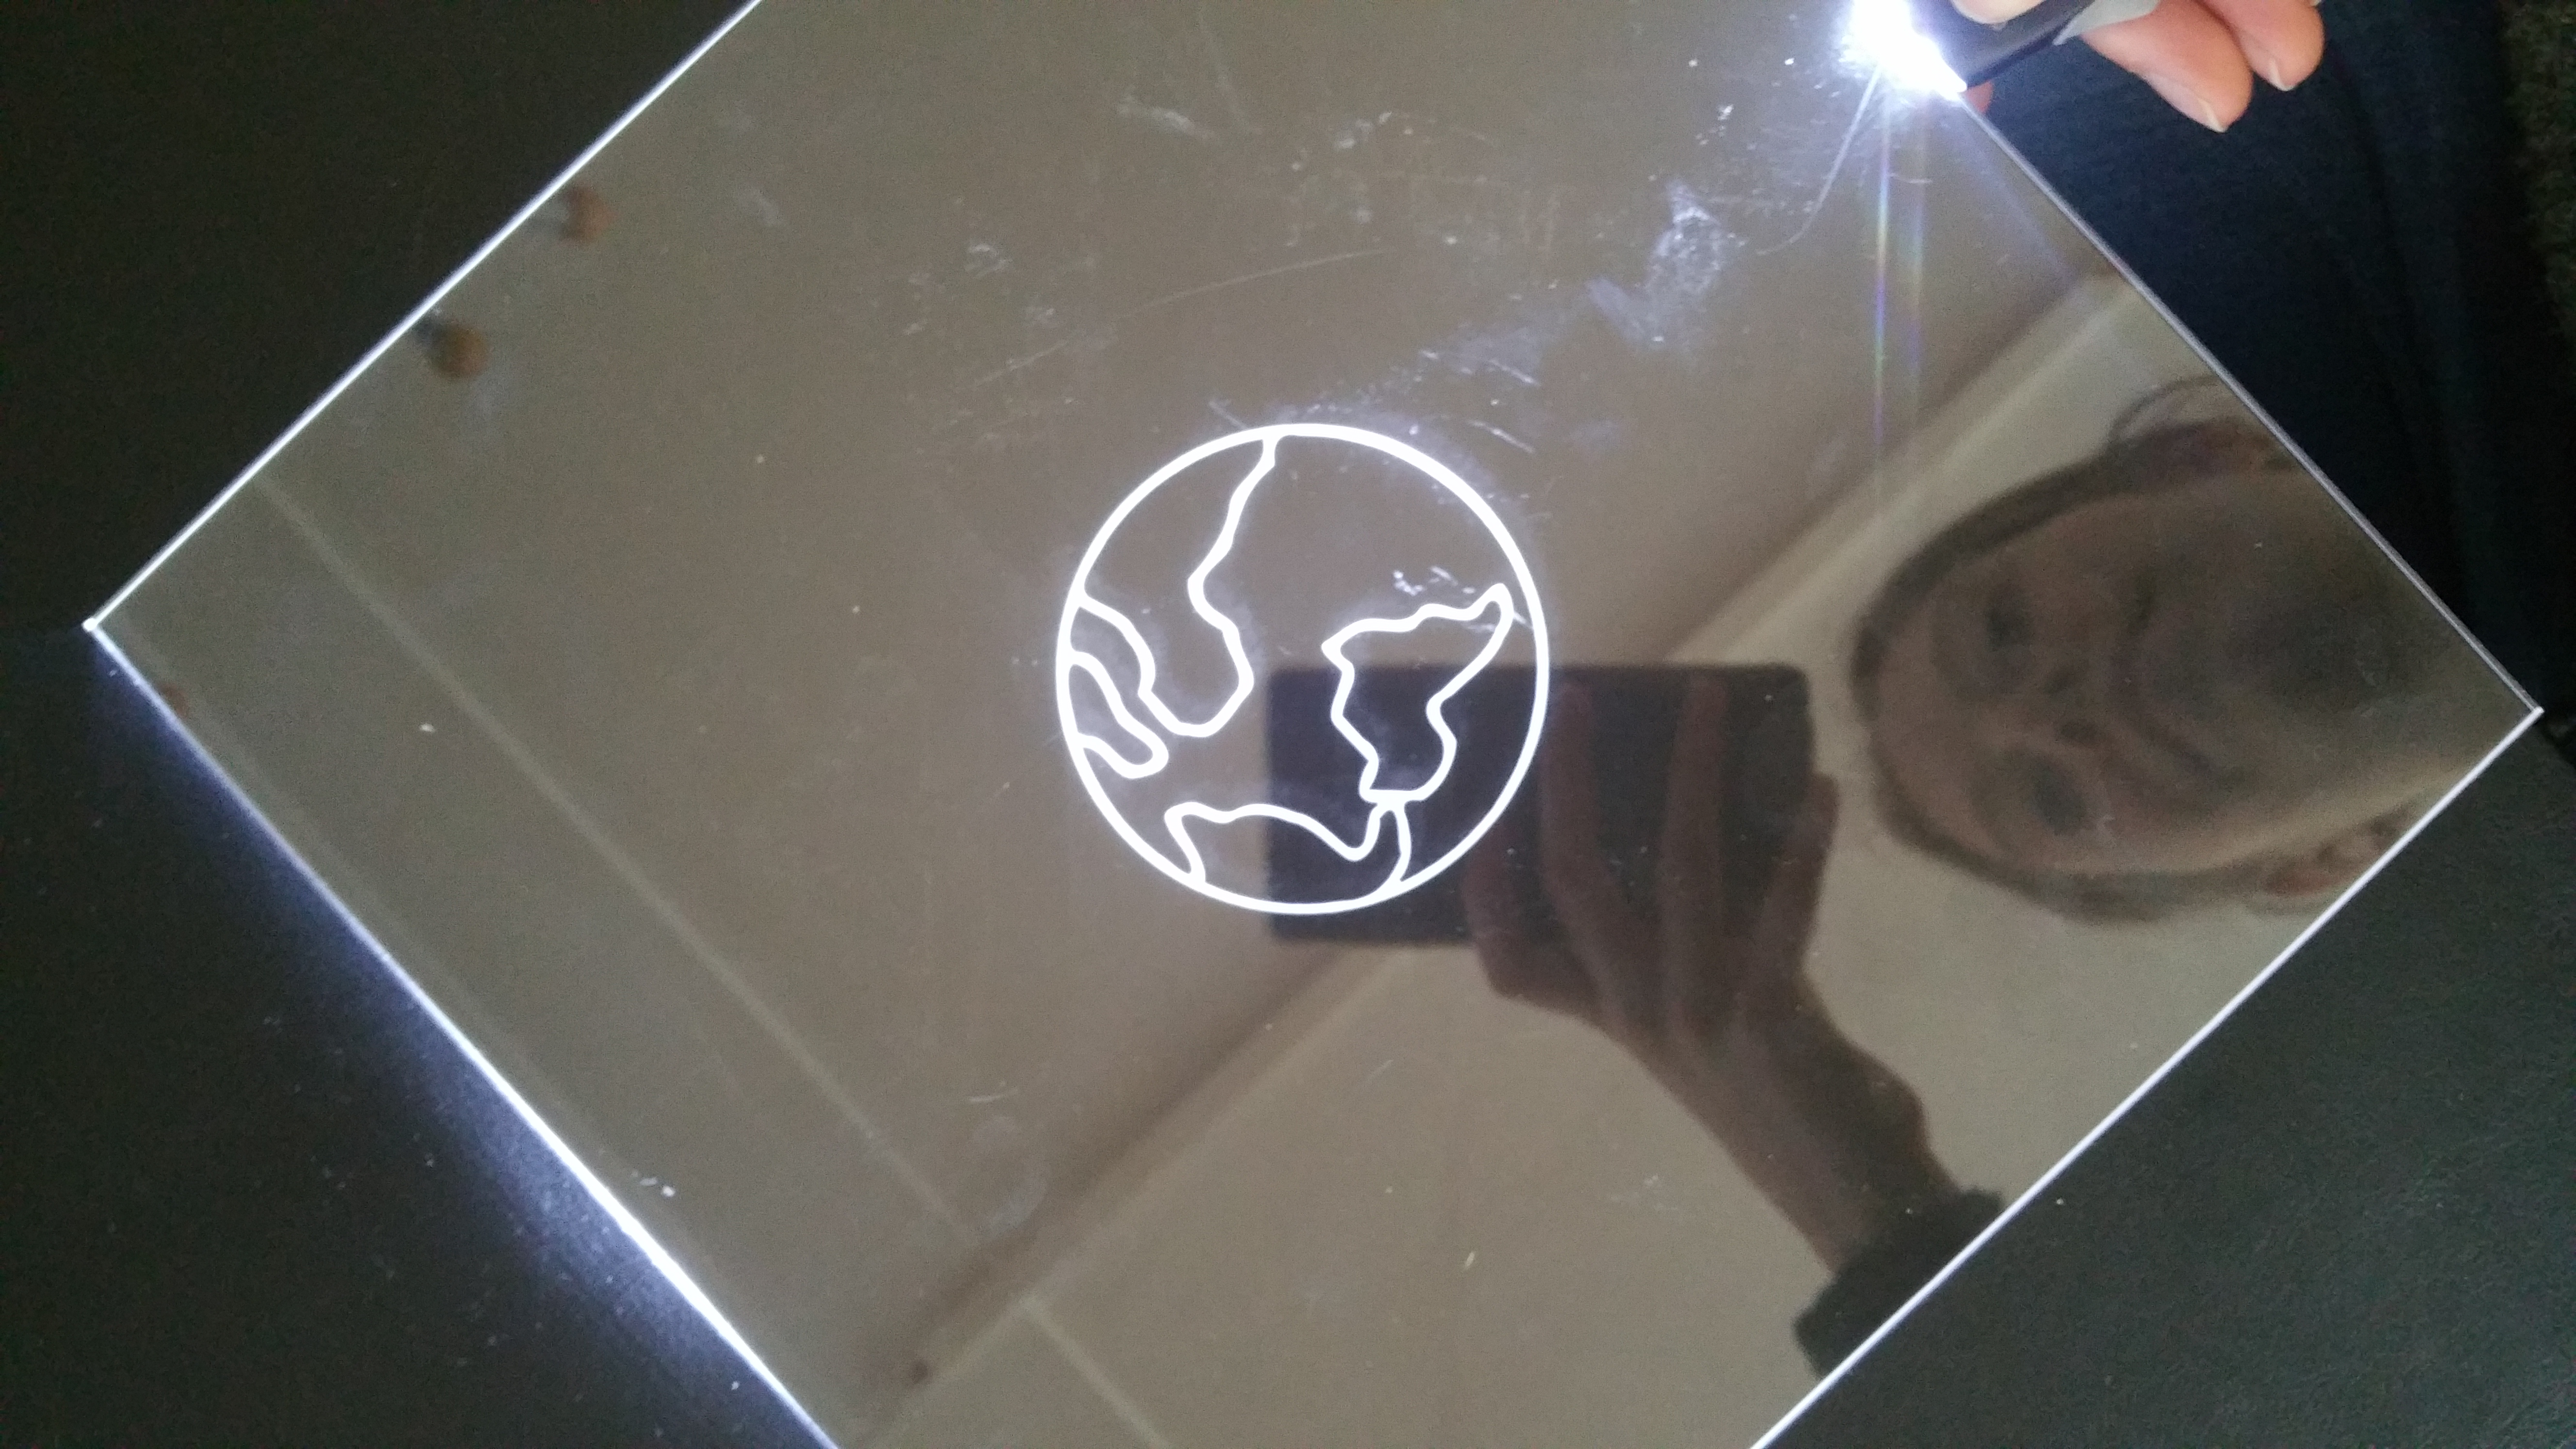
\includegraphics[width=0.6\textwidth]{img/PlexiPlaat.jpg}
  \caption{Plexi scherm}
  \label{fig:plexiplaat}
\end{figure}

\subsection{Aansturing motor}
De schijf draait rond met behulp van een brushless DC-motor uit een harde schijf.
Om deze aan te sturen is een speciale ESC-module\footnote{ESC: Electronic Speed Control} nodig.

Deze modules zijn ontworpen voor gebruik in quadcopters en verwachten bijgevolg
een speciale aansturing.
Het nodige signaal is een vorm van PWM, met een frequentie van 50 of
\SI{60}{\hertz}
en een pulsbreedte tussen $1$ en \SI{2}{\milli\second}.
De PWM-modules die ingebouwd zitten in de microcontroller kunnen niet opereren
in deze frequenties en pulsbreedtelimieten,
het protocol werd dus volledig in software geïmplementeerd.
Zie figuur~\ref{fig:motorpwm} voor een beeld het geproduceerde signaal.

Het PWM signaal wordt op pin §D0§ naar buiten gebracht. De software implementatie
van het PWM signaal is met Timer/Counter3 in Clear Timer on Compare Match (CTC)
modus verwezenlijkt. In het register OCR3A wordt een waarde ingesteld, wanneer de \texttt{Timer/Counter}
deze waarde bereikt wordt de counter op nul gezet en wordt de interrupt §TIMER3_COMPA_vect§
aangevraagd. Er wordt in de interrupt service routine een nieuwe waarde ingesteld
in §OCR3A§ en de output bit op pin §D0§ wordt geflipt. Deze counter werd gekozen
vanwege zijn 16-bits resolutie.

Om nul procent vermogen aan te sturen moet het signaal 1ms hoog zijn, om het
maximale vermogen aan te sturen moet het signaal 2 ms hoog zijn. De Timer/Counter3
heeft een frequentie van \SI{2}{\mega\hertz}, dat is de \texttt{I/O} klok van \SI{16}{\mega\hertz} verschaald met
prescaler $8$. Een cijfervoorbeeld van het PWM signaal dat overeenkomt met \SI{0}{\percent}
motorvermogen is in tabel~\ref{tbl:PWM} zichtbaar.

\begin{table}
  \centering
  \begin{tabular}{rSS}
    \hline
    & {Klokslagen} & {Tijd (\si{\milli\second})}\\
    \hline
    Hoge puls & 2000 & 1\\
    Lage puls & 38000 & 19\\
    \hline
    Periode & 40000 & 20\\
    \hline
  \end{tabular}
  \caption{PWM generatie}
  \label{tbl:PWM}
\end{table}

\begin{figure}
  \centering
  \includegraphics[width=0.6\textwidth]{img/scoopcontrolesc.png}
  \caption{Controlesignaal ESC}
  \label{fig:motorpwm}
\end{figure}

Een extra moeilijkheid is de opstartprocedure van de ESC.
De microcontroller moet opgestart zijn en een signaal sturen dat overeen komt
met \SI{0}{\percent} motorvermogen wanneer de ESC stroom krijgt en wordt
ingeschakeld. De ESC produceert dan een serie tonen, gevolgd door een langere
toon wanneer het signaal herkend wordt. Daarna kan de motor aangestuurd worden
en het vermogen verhoogd, liefst langzaam gezien het hoge gewicht van de draaischijf.
Uiteindelijk zal de ESC een driefasig signaal naar de motor sturen, zoals
zichtbaar in figuur~\ref{fig:motoresc}.

\begin{figure}
  \centering
  \includegraphics[width=0.6\textwidth]{img/scoopesc.png}
  \caption{Spanning naar de motor}
  \label{fig:motoresc}
\end{figure}

Deze procedure maakt het moeilijk om microcontroller en ESC op één voeding te
laten werken. Door de grote stroom is het ook lastig om bijvoorbeeld de ESC te
schakelen met een transistor. Voorlopig moet de ESC manueel in de stekker
gestoken worden. De driver wacht daartoe even met het opstarten van de motor,
aangezien de stekker pas mag ingeplugd worden wanneer het stuursignaal reeds
aanwezig is.

\subsection{Toerenteller schijf}
De hoeksnelheidsmeting component uit figuur 1 levert de hoeksnelheid en een
ijkpunt van de draaibeweging van de schijf. Als input krijgt de component een
puls van een stationaire optische sensor die gemonteerd is langs de rand van de
schijf. In de schijf zit een gaatje waardoor de optische sensor getriggerd wordt
als dit gaatje doorheen de sensor passeert. (Figuur~\ref{fig:sensor})

\begin{figure}
  \centering
  \includegraphics[width=0.6\textwidth]{img/Sensor.jpg}
  \caption{Sensor gemonteerd aan de rand van de schijf}
  \label{fig:sensor}
\end{figure}

De praktische realisatie berust op de Input Capture unit van Timer/Counter1.
Dit vereist de alternate function van poort §PD4§, namelijk §ICP1§ of Timer/Counter1
Input Capture Trigger. Als een dalende of stijgende flank (dit is vrij te kiezen)
geregistreerd wordt op pin §ICP1§ dan wordt de huidige waarde van Timer/Counter1
zo snel mogelijk gekopieerd in een register genaamd §ICR1§, waarna dat op zijn beurt
kan bevraagd worden door de microcontroller. Doordat een noise-canceling optie aanstaat duurt
het kopiëren vier systeemklokpulsen langer, wat geen probleem levert voor de
accuraatheid.

De frequentie waarop Timer/Counter1 telt is \SI{250}{\kilo\hertz}. Dit is de \texttt{I/O} klok van \SI{16}{\mega\hertz}
verschaald met prescaler 64.

De Input Capture unit heeft de mogelijkheid tot het genereren van een interrupt.
Indien ingesteld, wordt zodra de waarde in §ICR1§ gekopieerd is, de interrupt
aangevraagd. In de interrupt routine wordt eerst de opgevangen waarde gekopieerd
en vervolgens wordt met de waarde de tijd die verstreken is sinds de vorige interrupt
bepaald. De eenheid van deze waarde is nog arbitrair om de hoge resolutie te bewaren,
het is een verschaalde versie van het aantal increments.

De Timer/Counter1 overflow interrupt wordt getriggerd wanneer de maximale waarde
bereikt is en de telwaarde op nul wordt gezet. Elke keer dat de overflow vector
getriggerd wordt moet het aantal increments met $216$ verhoogd worden.

In tabel~\ref{tbl:toerental} is een meting van het aantal increments te zien. Voor een hoeksnelheid van 19 toeren per seconde
is het aantal increments \num{12870}. Elke \num{65536} increments vind een overflow plaats.
De verhoudingen tussen kloksnelheid en schijfsnelheid zijn dus goed gedimensioneerd.

\begin{table}
  \centering
  \begin{tabular}{SSS}
    \hline
    {Tijd per increment (\si{\micro\second})} & {Aantal increments} & {Hoeksnelheid (toeren/s)}\\
    \hline
    4 & 12870 & 19.42502\\
    \hline
  \end{tabular}
  \caption{Meting en berekening toerental}
  \label{tbl:toerental}
\end{table}

\subsection{Joysticks}
De beide joysticks zijn relatief eenvoudig om uit te lezen.
Ze bestaan telkens uit vier NO schakelaars, één per richting.
Aangezien elke joystick op een aparte \emph{port} van de microcontroller
aangesloten is, kan met een simpele §NOT§ operatie en enkele bitshifts een
consistente weergave gegenereerd worden, met 1 bit per richting die hoog is
wanneer de schakelaar actief is. Hiertoe moeten ook de pullups geactiveerd
worden. De driver voor de joysticks controleert ook welke schakelaars sinds de
laatste tick actief zijn geworden, en slaat deze apart op.

Enkele gemaksfuncties werden toegevoegd om uit deze bitweergave te bepalen of
een gekozen richting actief is.

\subsection{Game engine}
Intern wordt alles dat moet weergegeven worden, voorgesteld door een
\emph{entity}, dit zijn bijvoorbeeld kogels en spelers. Een \emph{entity} bevat
telkens informatie over de positie, in poolcoördinaten, en LED-informatie. De
meeste \emph{entities} bevatten ook extra informatie die intern nodig is, zoals
de levenskracht van een speler.

De game engine werkt op een relatief eenvoudig principe.
Op regelmatige basis wordt de functie §uint8_t tick(uint16_t time_since_zero)§
opgeroepen, deze voert enkele stappen uit:
\begin{enumerate}
\item \emph{Tick alle entities}, entities hebben een §tick()§ functie,\\
  bijvoorbeeld §player_tick(Player *p)§, die ervoor zorgt dat de entity zich
  verplaatst volgens zijn snelheid en eventueel reageert op invoer.

\item \emph{Controleer voor botsingen}, in deze stap wordt getest of er
  kogels een schip geraakt hebben, en eventueel levens van deze speler worden
  afgenomen.

\item \emph{Check voor het einde van het spel} door te controleren of beide
  spelers nog in leven zijn. Dit bepaalt de returnwaarde van deze functie,
  §true§ wanneer het spel moet verder gaan, anders §false§.
\end{enumerate}

Deze functie wordt aan \SI{30}{\hertz} opgeroepen, met behulp van
Timer/Counter0 in \emph{CTC} mode. De counter geeft dan een interrupt
telkens een ingestelde waarde wordt bereikt en begint vervolgens weer vanaf nul
te tellen. Voorlopig telt de counter tot \num{255}, indien mogelijk kan dit
later verlaagd worden om het spel sneller te maken.
De 8-bits resolutie is meer dan genoeg om een vrij
groot bereik van mogelijke frequenties te bereiken met de prescaler op de
maximale waarde van $1024$.

Alle kogels die op een moment in het spel zijn, worden weergegeven in een array
met vaste grootte, momenteel is dit de willekeurig gekozen waarde 20. Wanneer
er dus al 20 kogels in het spel zijn en een speler probeert te schieten, zal de
oudste kogel verwijderd worden, en vervangen door een nieuwe. Om te voorkomen
dat kogels te lang blijven rondvliegen, hebben ze een maximale levensduur,
wanneer deze op nul komt, verdwijnt de kogel. Uiteindelijk willen we kogels
langzaam laten donkerder worden wanneer ze deze limiet bereiken. Ze zakken apart
daarvan langzaamaan naar beneden.

\section{Openstaande Problemen}
Er is nog wat werk aan de fysieke constructie van de schijf en we twijfelen nog
over het aantal sectoren. Een groot deel van de code, zoals de \emph{game
  engine} en de driver voor LED-timing, is dus nog niet getest.
Dit testen en debuggen zal waarschijnlijk nog vrij veel tijd innemen.
Verder zijn er nog enkele verbeteringen te maken in de \emph{game engine},
zo wordt er nog geen melding gegeven wanneer een speler sterft en kan het spel
niet herstart worden zonder de microcontroller te resetten.
Het spel begint ook van zodra de controller opstart, in plaats van wanneer de
spelers klaar zijn. Dit is geen wenselijke werking.

\todo{openstaande problemen uitbreiden}

\section{Taakverdeling en Samenwerking}
De motordriver werd geschreven door Marieke. Zij schreef ook de code die voor de
juiste timing zorgt en de optische sensor uitleest en ontwierp en bouwde de behuizingen.

De game engine en aansturing van LED's werd gedaan door Stef,
net zoals uitlezen van joysticks en debugfunctionaliteit.

Onze samenwerking gebeurt via Git en
GitHub\footnote{\url{https://github.com/Epse/MCU_Project_PlanetFight}}. Taken worden
verdeeld via \emph{issues} op GitHub. Iedereen werkt aan een apart deel van de
code of de hardware, die regelmatig samen worden gezet.

\section{Conclusie en Toekomstig Werk}
Voor de specificatie van het project, zie tabel~\ref{tbl:specs}.
Dit project is bijzonder ambitieus, zeker voor een team bestaande uit twee
personen.
\todo{Alle ``voor als we tijd over hebben'' dingen opschrijven.}

\begin{table}
  \centering
  \begin{tabular}{l|c}
    \hline
    Parameter & Waarde\\
    \hline
    Ingangsspanning Microcontroller & \SI{5}{\volt}\\
    Ingangsspanning ESC & \SI{12}{\volt}\\
    Aantal spelers & 2\\
    Bediening & 2 Joysticks, 4 schakelaars elk\\
    Minimale updatefrequentie & \SI{24}{\hertz}\\
    Weergave & 15 LED's\\
    Radiale resolutie & 13\\
    Omtrekresolutie & 1024\\
    \hline
  \end{tabular}
  \caption{Specificaties}
  \label{tbl:specs}
\end{table}

\end{document}
